\documentclass[a4paper,12pt]{article}	% тип документа

\usepackage[a4paper,top=1.3cm,bottom=2cm,left=1.5cm,right=1.5cm,marginparwidth=0.75cm]{geometry} % field settings

\usepackage[T2A]{fontenc}		% кодировка
\usepackage[utf8]{inputenc}		% кодировка исходного текста
\usepackage[english,russian]{babel}	% локализация и переносы
\usepackage{indentfirst}

%Piece of code
\usepackage{listings}
\usepackage{xcolor}
\lstset
{
    language=C++,
    backgroundcolor=\color{black!4}, % set backgroundcolor
    basicstyle=\footnotesize,% basic font setting
}

%Drawings
\usepackage{graphicx}

\usepackage{wrapfig}

\usepackage{multirow}

\usepackage{float}

\usepackage{wasysym}

\usepackage[T1]{fontenc}
\usepackage{titlesec}

\setlength{\parindent}{3ex}

%Quatation
\usepackage{csquotes}

% Literature
\addto\captions{\def\refname{Literatur.}}

%Header
\title{
	\center{\textbf{Seminar 18.}}
	}


\begin{document}	% the beginning of the document

\maketitle

\section{Как организована иерархия классов потоков в библиотеке IOStream?}

	Иерархия классов потоков в библиотеке IOStream (все классы, кроме "родоначального" ios\_base имеют специализации для char и wchar\_t, обозначенные с использованием typedef; в то же время на данный момент отсутствуют специализации для типов char16\_t и char32\_t):
	
	\begin{itemize}
	
		\item Существует базовый класс, ios\_base, определяющий общие возможности и функциональность всех потомков: он задаёт состояние потока и флаги потока.
		
		\item Напрямую от ios\_base наследуется шаблонный класс basic\_ios<>, предоставляющий некоторые средства интерфейса для взаимодействия с объектами.
		
		\item Наследниками (динамический полиморфизм) basic\_ios<> являются basic\_istream<> и basic\_ostream<>, которые обеспечивают поддержку высокоуровневых операций ввода и вывода (соответственно) над символьными потоками: поддерживаемые операции включают форматированный и неформатированный ввод и вывод.
		
		\item От этих двух классов наследуется basic\_iostream<>, объединяющий многие возможности родителей. 
		
		\item От классов basic\_istream<>, basic\_ostream<> и basic\_iostream<> наследуются  basic\_istringstream<>, basic\_ostringstream<> и basic\_stringstream<> соответственно для работы со строками, а также basic\_ifstream<>, basic\_ofstream<> и basic\_fstream<> соответственно для работы с файлами.
	
	\end{itemize}
	
	Кроме того, важной частью библиотеки IOStream является класс basic\_streambuf<> и его наследники basic\_stringbuf<> и basic\_filebuf<>. Класс basic\_streambuf управляет вводом и выводом последовательностей символов: обеспечивает доступ к управляемой последовательности символов, называемой буфером, которая может содержать входную последовательность для буферизации операций ввода и/или выходную последовательность для буферизации операций вывода; а также обеспечивает доступ к связанной последовательности символов,  называемой источником (для ввода) или приёмником (для вывода). Это может быть объект, доступ к которому осуществляется через API ОS (например, файл) или это может быть объект (std::vector, массив, строковый литерал), который можно интерпретировать как источник или накопитель символов. Объекты потока ввода-вывода basic\_istream и basic\_ostream, а также все производные от них объекты полностью реализованы в терминах basic\_streambuf.
	
	Более удобными для восприятия иерархии являются рисунки \eqref{fig1} и \eqref{fig2}.
	
	\begin{figure}[h!]
		\begin{center}
			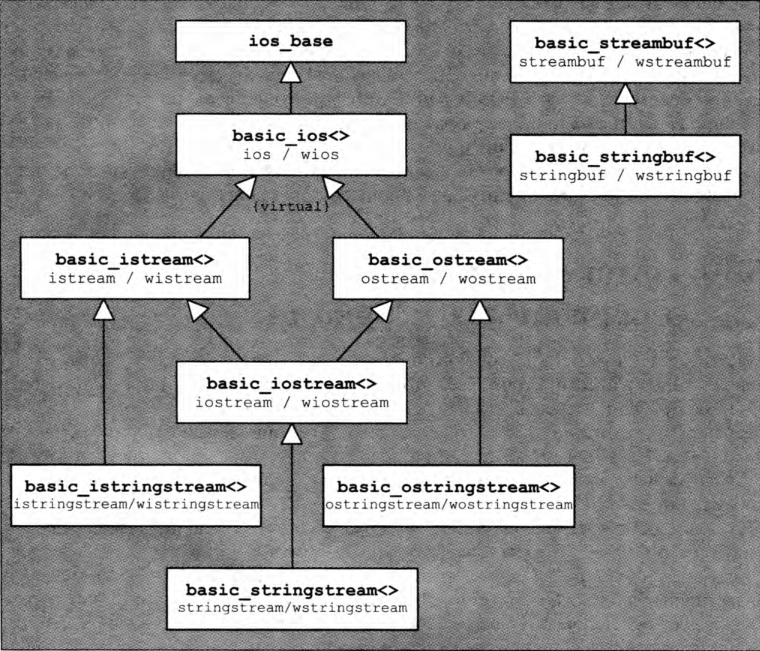
\includegraphics[scale = 0.4]{fig1}
			\caption{Иерархия классов потоков в библиотеке IOStream.}
			\label{fig1}
		\end{center}
	\end{figure}
	
	\begin{figure}[h!]
		\begin{center}
			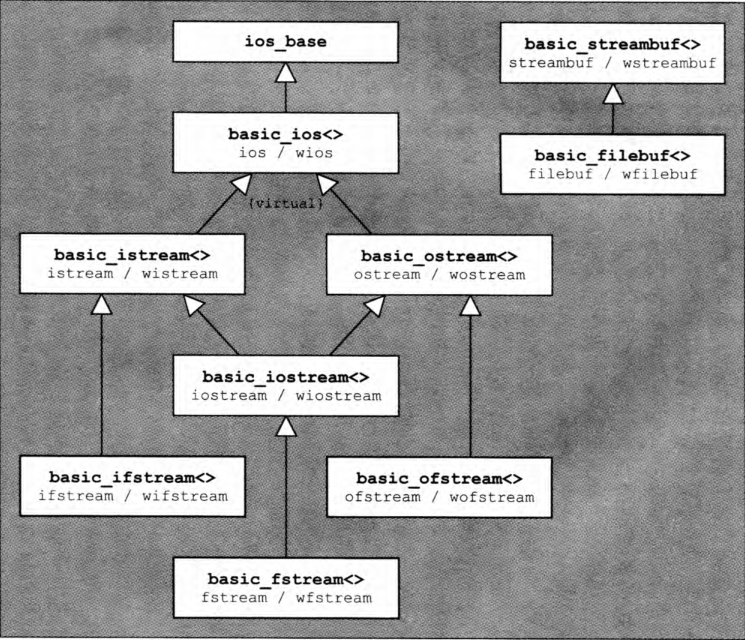
\includegraphics[scale = 0.4]{fig2}
			\caption{Иерархия классов потоков в библиотеке IOStream.}
			\label{fig2}
		\end{center}
	\end{figure}

\section{Какие состояния потоков реализованы в базовом классе basic\_ios?}

	Состояния потоков, реализованые в базовом классе basic\_ios:
	
	\begin{itemize}
	
		\item good bit -- всё в порядке;
		
		\item eofbit -- конец файла;
		
		\item failbit -- сбой при вводе/выводе (не фатальная ошибка);
				
		\item badbit -- фатальная ошибка.	
	
	\end{itemize}

	Стоит отметить, что в случая сбоя в потоке его состояние нужно сбрасывать вручную, с помощью clear.

\section{В чём разница между манипуляторами и флагами форматирования?}

	Манипуляторы -- это вспомогательные функции, управляющие потоком данных обычно локально (т.е. в рамках одной команды, в месте использования operator>>/operator<<). Флаги форматирования же позволяют делать глобальные настройки для каких-либо потоков (т.е. эти настройки будут сохраняться для данного потока на протяжении выполенния всей программы после настройки/до новых изменений флагов). Т.о., флаги и манипуляторы выполняют одну и туже задачу -- задают определённый формат ввода-вывода информации в потоках, но используются по-разному.

\section{Из каких основных элементов состоят пути в файловой системе?}

	Путь -- набор символов, показывающий расположение файла или каталога в файловой системе. Пути могут быть абсолютными или относительными в зависимости от наличия тех или иных компонент. Основные элементы пути:
	
	\begin{itemize}
	
		\item Названия корня (в зависимости от типа пути), директории/ий (каталоги) и файла.
	
		\item Разделительный знак. В OS UNIX разделительным знаком при записи пути является (/), в Windows -- ($\backslash$) (обычно). Эти знаки служат для разделения названия каталогов, составляющих путь к файлу. Кроме того, в случае Windows может быть также использован  разделитель томов (:) для формирования абсолютного пути к файлу из корня диска. Также в Windows существуют разделители (.) и (..).
	
		\item Кодировка имени файла. В Unix/Linux имя файла представляет собой последовательность любых байтов, кроме косой черты или NUL. Современные среды Unix/Linux прекрасно обрабатывают имена файлов в кодировке UTF-8. В Windows для этих целей используется UTF-16. Это определяет использование типов char и wchar\_t в Linux и Windows соответственно. 
	
	\end{itemize}
	

\section{Зачем нужны форматы обмена данными, такие как JSON и XML?}

	Форматы обмена данными удобны для чтения и написания как человеком, так и компьютером. С их помощью успешно создаётся разметка в документах и текстах, где доля разнотипных символьных данных велика, а доля разметки мала. Более того, форматы обмена данными не зависят от языка программирования и часто основываются на универсальных структурах данных, поддерживаемых многими современными языками программирования в какой-либо форме. В частностти, они позволяют лаконично производить сериализацию и десериализацию (при передаче объектов по сети и для сохранения их в файлы).

			
\newpage

	
\addcontentsline{toc}{section}{Literature}
 
	\begin{thebibliography}{}
	
		\bibitem{litlink1} https://en.cppreference.com/w/
		\bibitem{litlink2} https://www.json.org/json-en.html
		
	\end{thebibliography}


\end{document} % end of the document
